\documentclass{llncs}
%\documentclass{elsart}
%\usepackage{fullpage,epsfig,latexsym,pst-tree,scalefnt}
\usepackage{epsfig,latexsym,pst-tree,scalefnt}
\setlength{\headsep}{.4in}
\parskip 6pt

\def\rsy{respectively}
\def\at{autotree}
\def\impt{implicit tree}
\def\stt{strategy tree}
\def\aot{and/or tree}
\def\aoat{and/or autotree}
\def\gt{gametree}
\def\bpsn{board position}
\def\exct{excised tree}
%\def\str{strategy}
\def\myAND{\mbox{\tt and}}
\def\myOR{\mbox{\tt or}}
\def\andnode{\myAND-node}
\def\ornode{\myOR-node}
\def\calS{\mbox{$\mathcal S$}}
%\def\bs{board-state}
\def\gs{game-state}
%\def\sg{subgame}
\def\endofproof{\hfill $\Box$}
\newtheorem{theorem}{Theorem}
\newtheorem{corollary}[theorem]{Corollary}
\newtheorem{observation}[theorem]{Observation}
\newcommand{\board}[2]{\mbox{$#1$$\times$$#2$}}

%\newcommand{\tpl}[3]{\mbox{$#1$($#2$:$-,#3,-$)}}

\begin{document}
\begin{frontmatter}

%% possible Journal version title:
%%\title{Automatic strategy verification for the game of Hex}
\title{Verifying Hex strategies}\thanks{The 
support of NSERC is gratefully acknowledged.}

\author[A1]{Ryan~Hayward}
\author[A1]{Broderick~Arneson}
\author[A1]{Philip~Henderson}
\address[A1]{Department of Computing Science,
             University of Alberta,
             Edmonton, Alberta, Canada,
         \{hayward,broderic,ph\}@cs.ualberta.ca}

\begin{abstract}
We present a concise and/or-tree notation
%We present an and/or-tree notation
for describing Hex strategies
together with an easily implemented algorithm
for verifying strategy correctness.
%%Our notation is concise in that 
%%it allows independent substrategies to be expressed
%%using an ``and'' operator,
%%it allows repeated substrategies to be described
%%with a macro operator,
%%and it groups every set of opponent responses into a single meta-response.
%%
To illustrate our algorithm, we use it to verify 
Jing Yang's \board{7}{7} centre-opening strategy.
\end{abstract}

\begin{keyword}
Hex, strategy verification
\end{keyword}
\end{frontmatter}

\vspace*{-5in}
{\it submitted 22 Jan 2006 to CG 2006}
\vspace*{5in}

\begin{figure}[h]
{\scriptsize 
\ \hfill \epsfig{file=B3.eps} 
\ \hfill \epsfig{file=B3full.eps} 
\hfill \  
}
\caption{The start (left) and finish (right) of a Hex game on a 
\board{3}{3} board.}
%%for the strategy of Fig.~\ref{fig:T3x3}.}
\label{fig:B3}
\end{figure}


\section{Introduction}

An intriguing aspect of the game of Hex\footnote{
  Hex is the classic two-player board game invented by Piet Hein in
  1942 and independently by John Nash around 1948 
  \cite{Nash52,Gardner57,Gardner59,Maarup05,Maarup05w,Nasar98}.
  The game is named after the board,
  which consists of a parallelogram-shaped $m$$\times$$n$ array of
  hexagons, also called cells. 
  Each player is assigned a set of
  stones and two opposing board sides;
  players alternately place a stone on an unoccupied cell; 
  the first player to form a path connecting her two sides
  with her stones wins the game.
  For example,  Fig.~\ref{fig:B3},
  shows the start and end of a game on a \board{3}{3} board.
  White succeeds in joining her two sides, so White wins this game.
  For more on Hex, see the recent survey by 
  Hayward and Van Rijswijck \cite{HaywardvanR05}
  or the web page by Thomas Maarup \cite{Maarup05w}.}
is that for all \board{n}{n} boards,
although a winning first-player strategy is known to exist
\cite{Nash52,Gardner57,Gardner59},
explicit such strategies have been found only for small boards.
While finding such strategies is routine on very small boards,
the task quickly becomes challenging as board size increases.
This is not surprising since, as Stefan Reisch has shown, 
determining the winner of arbitrary Hex positions is PSPACE-complete
\cite{Reisch81}.

For \board{7}{7}, \board{8}{8}, and \board{9}{9} boards,
Jing Yang found strategies by hand \cite{Yang01,Yang02a,Yang02b,Yang03}.
Later, Hayward et al.~found other \board{7}{7} strategies by computer 
\cite{HaywardEtAl03,HaywardEtAl05},
while Noshita found \board{7}{7} strategies
and one \board{8}{8} strategy similar to Yang's by hand \cite{Noshita05}.
For boards \board{10}{10} or larger, no winning strategies are known.

As the search for winning strategies on larger boards continues,
it is of interest to provide algorithms 
for verifying strategy correctness.
Recently, Noshita described strategies in a manner 
that arguably facilitates human verification \cite{Noshita05}.
By contrast, in this paper we present 
a system that allows for computer verification.
To demonstrate the utility of our system, we use it to
confirm the correctness of Yang's original \board{7}{7} strategy \cite{Yang01}.

\section{Excised trees and \at s}
The key feature of our verification system is
the tree notation we use to represent strategies.\footnote{This 
  notation could also be used for other two-player board games
  in which game pieces do not move once they have been placed.}
Our notation allows the standard tree description 
of a strategy to be condensed in three ways.
Firstly, it permits the use of an ``and'' operation
corresponding to the combinatorial sum of independent substrategies.
Secondly, it permits the use of a macro descriptor for representing
repeatedly occurring substrategies.
Thirdly, it allows 
all opponent moves to be excised from the notation by replacing 
each set of opponent responses with a single anonymous meta-response.

The first two of these three ideas are well known;
for example, they were used by Yang in his description
of his proofs \cite{Yang01,Yang02a,Yang02b,Yang03}.
The third idea, namely using \exct s, is new.
In the rest of this section we
illustrate the excision process and
show that it does not hamper verification.

\begin{figure}[t]
\ \hfill
{\tiny
%{\pstree[treesep=1pt,nodesep=1pt,treefit=tight,levelsep=8ex]{ \TR{c1} } {
{\pstree[linewidth=0pt,treesep=1pt,nodesep=1pt,treefit=tight,levelsep=8ex]{ \TR{c1} } {
   \pstree{ \TR{a1} } {
     \pstree{ \TR{c2} } {
       \pstree{\TR{a2}}{\TR{c3}}
       \pstree{\TR{a3}}{\TR{c3}}
       \pstree{\TR{b1}}{\TR{c3}}
       \pstree{\TR{b2}}{\TR{c3}}
       \pstree{\TR{b3}}{\TR{c3}}
       \pstree{\TR{c3}}{\TR{b3}}
     }
   }
   \pstree{ \TR{a2} } {
     \pstree{ \TR{c2} } {
       \pstree{\TR{a1}}{\TR{c3}}
       \pstree{\TR{a3}}{\TR{c3}}
       \pstree{\TR{b1}}{\TR{c3}}
       \pstree{\TR{b2}}{\TR{c3}}
       \pstree{\TR{b3}}{\TR{c3}}
       \pstree{\TR{c3}}{\TR{b3}}
     }
   }
   \pstree{ \TR{a3} } {
     \pstree{ \TR{c2} } {
       \pstree{\TR{a1}}{\TR{c3}}
       \pstree{\TR{a2}}{\TR{c3}}
       \pstree{\TR{b1}}{\TR{c3}}
       \pstree{\TR{b2}}{\TR{c3}}
       \pstree{\TR{b3}}{\TR{c3}}
       \pstree{\TR{c3}}{\TR{b3}}
     }
   }
   \pstree{ \TR{b1} } {
     \pstree{ \TR{c2} } {
       \pstree{\TR{a1}}{\TR{c3}}
       \pstree{\TR{a2}}{\TR{c3}}
       \pstree{\TR{a3}}{\TR{c3}}
       \pstree{\TR{b2}}{\TR{c3}}
       \pstree{\TR{b3}}{\TR{c3}}
       \pstree{\TR{c3}}{\TR{b3}}
     }
   }
   \pstree{ \TR{b2} } {
     \pstree{ \TR{c2} } {
       \pstree{\TR{a1}}{\TR{c3}}
       \pstree{\TR{a2}}{\TR{c3}}
       \pstree{\TR{a3}}{\TR{c3}}
       \pstree{\TR{b1}}{\TR{c3}}
       \pstree{\TR{b3}}{\TR{c3}}
       \pstree{\TR{c3}}{\TR{b3}}
     }
   }
   \pstree{ \TR{b3} } {
     \pstree{ \TR{a3} } {
       \pstree{\TR{a1}}{\TR{b2}}
       \pstree{\TR{a2}}{\TR{b2}}
       \pstree{\TR{b1}}{\TR{b2}}
       \pstree{\TR{b2}}{
         \pstree{\TR{a2}}{
	   \pstree{\TR{a1}}{\TR{b1}}
	   \pstree{\TR{b1}}{\TR{a1}}
	   \pstree{\TR{c2}}{\TR{a1}}
	   \pstree{\TR{c3}}{\TR{a1}}
         }
       }
       \pstree{\TR{c2}}{\TR{b2}}
       \pstree{\TR{c3}}{\TR{b2}}
     }
   }
   \pstree{ \TR{c2} } {
     \pstree{ \TR{b2} } {
       \pstree{\TR{a1}}{\TR{a3}}
       \pstree{\TR{a2}}{\TR{a3}}
       \pstree{\TR{a3}}{\TR{b3}}
       \pstree{\TR{b1}}{\TR{a3}}
       \pstree{\TR{b3}}{\TR{a3}}
       \pstree{\TR{c3}}{\TR{a3}}
     }
   }
   \pstree{ \TR{c3} } {
     \pstree{ \TR{b2} } {
       \pstree{\TR{a1}}{\TR{a3}}
       \pstree{\TR{a2}}{\TR{a3}}
       \pstree{\TR{a3}}{\TR{b3}}
       \pstree{\TR{b1}}{\TR{a3}}
       \pstree{\TR{b3}}{\TR{a3}}
       \pstree{\TR{c2}}{\TR{a3}}
     }
   }
}
}}\hfill \ 
\caption{A winning first-player \board{3}{3} Hex strategy.
Fig.~\ref{fig:B3} shows one line of this strategy.}
\label{fig:T3x3}
\end{figure}


To begin, consider the first-player \stt\ in Fig.~\ref{fig:T3x3}.
The nodes at even depth indicate first-player moves;
the nodes at odd depth indicate second-player moves;
the game in Fig.~\ref{fig:B3} 
follows one root-to-leaf path through the tree.
Notice that the first-player strategy
described by the tree is {\it complete}:
after each second-player move,
there is a unique first-player response;
after each first-player move,
there is every possible second-player response.
Also,
each leaf node establishes a first-player win,
so this is a winning strategy for the first player.

\begin{figure}[t]
\ \hfill
{\scriptsize
%{\pstree[treesep=0pt,nodesep=1pt,treefit=tight,levelsep=6ex]{ \TR{c1} } {
{\pstree[linewidth=0pt,treesep=0pt,nodesep=1pt,treefit=tight,levelsep=6ex]{ \TR{c1} } {
   \pstree{ \TR{$\bullet$} } {
     \pstree{ \TR{c2} } {
       \pstree{\TR{$\bullet$}}{
         \TR{c3}
         \TR{c3}
         \TR{c3}
         \TR{c3}
         \TR{c3}
         \TR{b3}
       }
      }
     \pstree{ \TR{c2} } {
       \pstree{\TR{$\bullet$}}{
         \TR{c3}
         \TR{c3}
         \TR{c3}
         \TR{c3}
         \TR{c3}
         \TR{b3}
       }
      }
     \pstree{ \TR{c2} } {
       \pstree{\TR{$\bullet$}}{
         \TR{c3}
         \TR{c3}
         \TR{c3}
         \TR{c3}
         \TR{c3}
         \TR{b3}
       }
      }
     \pstree{ \TR{c2} } {
       \pstree{\TR{$\bullet$}}{
         \TR{c3}
         \TR{c3}
         \TR{c3}
         \TR{c3}
         \TR{c3}
         \TR{b3}
       }
      }
     \pstree{ \TR{c2} } {
       \pstree{\TR{$\bullet$}}{
         \TR{c3}
         \TR{c3}
         \TR{c3}
         \TR{c3}
         \TR{c3}
         \TR{b3}
       }
      }
      \pstree{ \TR{a3} } {
         \pstree{\TR{$\bullet$}}{
           \TR{b2}  
           \TR{b2}  
           \TR{b2}  
	   \pstree{\TR{a2}}{
	      \pstree{\TR{$\bullet$}} {
	         \TR{b1}
	         \TR{a1}
	         \TR{a1}
	         \TR{a1}
              }
           }
           \TR{b2}  
           \TR{b2}  
         }
       }
       \pstree{ \TR{b2} } {
         \pstree{\TR{$\bullet$}}{
           \TR{a3}
           \TR{a3}
	   \TR{b3}
           \TR{a3}
           \TR{a3}
           \TR{a3}
         }
       }
       \pstree{ \TR{b2} } {
         \pstree{\TR{$\bullet$}}{
           \TR{a3}
           \TR{a3}
	   \TR{b3}
           \TR{a3}
           \TR{a3}
           \TR{a3}
         }
       }
     }
   }
}}\hfill \ 

\vspace*{-.3in}
{\scriptsize
\ \hfill
%{\pstree[treemode=R,treesep=7pt,nodesep=1pt,treefit=tight,levelsep=8ex]{ \TR{c1} } {
{\pstree[linewidth=0pt,treesep=1pt,nodesep=1pt,treefit=tight,levelsep=6ex]{ \TR{c1} } {
   \pstree{ \TR{$\bullet$} } {
     \pstree{ \TR{c2} } {
       \pstree{\TR{$\bullet$}}{
         \TR{c3}
         \TR{b3}
       }
      }
      \pstree{ \TR{a3} } {
         \pstree{\TR{$\bullet$}}{
           \TR{b2}  
	   \pstree{\TR{a2}}{
	      \pstree{\TR{$\bullet$}} {
	         \TR{b1}
	         \TR{a1}
              }
           }
         }
       }
       \pstree{ \TR{b2} } {
         \pstree{\TR{$\bullet$}}{
           \TR{a3}
	   \TR{b3}
         }
       }
     }
   }
}}\hfill \ 
\caption{The tree obtained from the \stt\ in Fig.~\ref{fig:T3x3}
by replacing each set of opponent response nodes with a 
single ``$\bullet$'' meta-node (top),
and the \exct\ obtained by then 
repeatedly merging identical subtrees (bottom).}
\label{fig:T3x3imp}
\end{figure}


Next, consider the two trees shown in Fig.~\ref{fig:T3x3imp}.
The top tree is obtained from the tree in Fig.~\ref{fig:T3x3}
by excising nodes corresponding to second-player moves;
each set of moves is replaced with a single meta-node,
indicated in our diagrams by a dot ($\bullet$).
The bottom tree is obtained from the top tree
by repeatedly merging identical subtrees into a single subtree
until, for each node, all subtrees are distinct.
We refer to the bottom tree as an {\it \exct}.

While some information is lost when a \stt\ is replaced with its \exct,
the excision process can be reversed in the following sense:
for any \exct\ $E$ for a player, 
there is a unique set \calS\ of \stt s 
such that $E$ is the \exct\ of every tree in \calS.
Furthermore, it is easy to construct elements of \calS\ from $E$
via the following process, which we call {\it restoration}:

\begin{quotation}{\it
\noindent
Proceed through $E$ in top-down order. At each meta-node $m$,
for each possible opponent move to a cell $c$,
select for the player's responding move any cell $r$
that is the root of a subtree of $m$ in which $c$ does not appear.
}\end{quotation}

For example, consider the restoration process
for the \exct\ shown in Fig.~\ref{fig:T3x3imp}.
We start with the top-most meta-node $m^*$,
namely the child of $c1$.
For this board position,
the cell set of possible opponent moves
is $\{a1$, $a2$, $a3$, $b1$, $b2$, $b3$, $c2$, $c3\}$.
Consider the first such cell, $a1$.
The cell sets of the subtrees of $m^*$ are 
$\{c2,b3,c3\}$,
$\{a3,b2,a2,b1,a1\}$, and
$\{b2,a3,b3\}$.
Since $a1$ is not in the first or third 
of these three cell sets, we can select
the root of either the first or third subtree of $m^*$.
Let us assume in this example that we always
select the root of the first available subtree.
Thus, as the response to $a1$ we select the root
of the first subtree, namely $c2$.
Continuing in this fashion, 
we select $c2$ as the response for
opponent moves to $a2$, $a3$, $b1$, $b2$,
and $a3$ as the response for opponent moves
to $b3$, $c2$, $c3$.
Having selected all responses to $m^*$,
we continue in top-down order to process meta-nodes
until all such nodes have been dealt with and the 
\exct\ has been replaced with a complete \stt\ $S'$ of \calS.

Notice that $S'$ is different from the \stt\ $S$
of Fig.~\ref{fig:T3x3} from which $E$ was derived,
as in the restoration process
we never selected the root of the third subtree of $m^*$
as a response to an opponent move.
However, by repeating the restoration once for each
of the possible permutations of choices for $r$,
we would construct all possible \stt s associated with $E$,
including $S$.

The restoration process is well defined in that it is always possible 
to find at least one value of $r$ at each meta-node.  
This follows from the next observation,
which in turn follows from the fact that in Hex, 
stones never move once played.

A $\pi$-move is a move made by player $\pi$;
a $\pi$-node is a node associated with a $\pi$-move.
The $\pi$-descendants of a subtree are all $\pi$-nodes in the subtree.

\begin{observation}
In a Hex \stt\ for a player $\pi$,
let $p$ be a $\pi$-node,
let $S_1$,\ldots,$S_t$ be the subtrees of $p$,
and for each $S_j$ let $P_j$ be the $\pi$-descendants of $S_j$.
Then the combined intersection $I=P_1\cap \ldots \cap P_t$ is empty.
\end{observation}

{\it Proof}.
For each $S_j$ let $c_j$ be the 
cell associated with the root of $S_j$.
Thus $c_j$ is a cell to which $\pi$'s opponent moved,
so $c_j$ is not in $P_j$ and so not in $I$.
This holds for all $c_j$ in $C=\{c_1,\ldots,c_t\}$,
where $C$ is the set of unoccupied cells after the $\pi$-move $p$.
Thus $I$ is empty.
\endofproof

The following is an immediate corollary of the preceding.

\begin{observation}\label{obs:elusive}
In an \exct\ of a Hex \stt\ for a player $\pi$,
for every meta-node $m$ that is not a leaf,
the combined intersection of the 
$\pi$-descendants of the subtrees of $m$ is empty.
\endofproof
\end{observation}

%%We denote by $(B,\pi)$ the \gs\ with \bpsn\ $B$ and player to move $\pi$.
%%We denote by $\overline{\pi}$ the opponent of $\pi$.
%%A $\pi$-move is a move made by $\pi$.
%%A $\pi$-node is a node in a \stt\ corresponding to a $\pi$-move.
%%A {\it \str} for a \gs\ $(B,\pi)$ is a strategy for that player and \bpsn,
%%namely for each \gs\ $(B',\pi)$ reachable from $(B,\pi)$,
%%all possible $\overline{\pi}$-moves are considered, and 
%%for each non-terminal \gs\ $(B'',\overline{\pi})$ one $\pi$-move is specified.
%%The {\it \stt} for a \str\ is the associated \gt,
%%namely each $\pi$-{\it node} has one child for each possible responding $\overline{\pi}$-move
%%and each non-leaf $\overline{\pi}$-node has one child.

We refer to the class of trees that we use
in our verification system as ``\at s'';
we use this term since such trees
make explicit mention only of a player's {\it own} moves.
Autotrees have the same form and function
as \exct s; however, they may not have arisen via excision, 
and so we do not define them with respect to excision.
An {\it \at} is defined as follows:
each node at one set of alternating levels is
a special node called a {\it meta-node};
each node at the other set of alternating levels has a cell label.

We call an \at\ {\it elusive}
if it satisfies the conditions of Observation~\ref{obs:elusive}.
Notice that the restoration generates a \stt\ from
an \at\ if and only if the \at\ is elusive.
As an initial step in our verification algorithm,
we check whether the input \at\ is valid,
namely whether it is elusive.

The second and final step in our verification algorithm
is to determine whether the strategies
associated with the input \at\ are winning.
We call an \at\ of a player
{\it satisfying} if, for every leaf,
the cells of the root-to-leaf path 
satisfy the conditions of a win,
namely join the player's two sides on the Hex board.
A valid \at\ represents a winning strategy
if and only if the \at\ is satisfying.
This follows from the following theorems,
which in turn follow by straightforward arguments from
our definitions and the discussion to this point;
we omit the details of the proofs.

\begin{theorem}
For any Hex \stt\ there is a unique associated \exct,
and for any \at\ there is a unique set of associated \stt s.
Furthermore, a \stt\ $S$ is winning if and only if
each \stt s $S'$ created via restoration
from the \exct\ derived from $S$ is winning.
\end{theorem}

\begin{theorem}
An \at\ represents a winning strategy if and only if
the \at\ is elusive and satisfying.
\end{theorem}

\section{And/or \at s with leaf patterns}
To complete the description of our notation,
we need only to describe how we add two features to \at s:
\andnode s and leaf patterns.

\begin{figure}[t]
\ \hfill
{\pstree[treemode=R,linewidth=1pt,treesep=4pt,nodesep=4pt,treefit=tight,levelsep=6ex]{ \TR{d1} } {
   \pstree{ \TR{$\bullet$} } {
     \pstree{ \TR{c3} } {
       \pstree{\TR{$\bullet$}}{
         \TR{b4}
         \TR{c4}
       }
       \pstree{\TR{$\bullet$}}{
         \TR{c2}
         \TR{d2}
       }
     }
     \pstree{ \TR{b3} } {
       \pstree{\TR{$\bullet$}}{
         \TR{a4}  
         \TR{b4}  
       }
       \pstree{\TR{$\bullet$}} {
         \pstree{\TR{a2}}{
           \pstree{\TR{$\bullet$}}{
             \TR{a1}  
             \TR{b1}  
           }
           \pstree{\TR{$\bullet$}}{
             \TR{a3}  
             \TR{b2}  
           }
         }
         \TR{c2}
       }
     }
     \pstree{ \TR{b3} } {
       \pstree{\TR{$\bullet$}}{
         \TR{a4}  
         \TR{b4}  
       }
       \pstree{\TR{$\bullet$}} {
         \pstree{\TR{b2}}{
           \pstree{\TR{$\bullet$}}{
             \TR{b1}  
             \TR{c1}  
           }
         }
         \pstree{\TR{d2}}{
           \pstree{\TR{$\bullet$}}{
             \TR{c3}  
             \pstree{\TR{d3}}{
               \pstree{\TR{$\bullet$}}{
                 \TR{c4}  
                 \TR{d4}  
               }
             }
           }
         }
       }
     }
     \pstree{ \TR{d3} } {
       \pstree{\TR{$\bullet$}}{
         \TR{c4}  
         \TR{d4}  
       }
       \pstree{\TR{$\bullet$}} {
         \TR{d2}
         \pstree{\TR{b3}}{
           \pstree{\TR{$\bullet$}} {
             \TR{a4}  
             \TR{c3}  
           }
           \pstree{\TR{$\bullet$}}{
             \TR{c2}  
             \pstree{\TR{a2}}{
               \pstree{\TR{$\bullet$}}{
                 \TR{a1}  
                 \TR{b1}  
               }
               \pstree{\TR{$\bullet$}}{
                 \TR{a3}  
                 \TR{b2}  
               }
             }
           }
         }
       }
     }
   }
 }
}\hfill \ 
%\caption{An \aoat\ for a winning first-player \board{4}{4} Hex strategy.
%Odd depth nodes ($\bullet$) are ``or''-nodes;
%even depth nodes (cell labels) are ``and''-nodes.
%Fig.~\ref{fig:B4} shows one line of this strategy.}
%\label{fig:T4x4}
\end{figure}


\ \hf \epsfig{file=B4.eps,scale=2.0}  \hf \ 

\vspace*{.5in}

\ \hfill \epsfig{file=B4full.eps,scale=2.0} \hf \ 

\vspace*{.5in}

\ \hfill
\pstree[treemode=R,linewidth=1pt,treesep=4pt,nodesep=4pt,treefit=tight,levelsep=6ex]{ \TR{d1} } {
   \pstree{ \TR{$\bullet$} } {
     \pstree{ \TR{c3} } {
       \pstree{\TR{$\bullet$}}{
         \TR{b4}
         \TR{c4}
       }
       \pstree{\TR{$\bullet$}}{
         \TR{c2}
         \TR{d2}
       }
     }
     \pstree{ \TR{b3} } {
       \pstree{\TR{$\bullet$}}{
         \TR{a4}  
         \TR{b4}  
       }
       \pstree{\TR{$\bullet$}} {
         \pstree{\TR{a2}}{
           \pstree{\TR{$\bullet$}}{
             \TR{a1}  
             \TR{b1}  
           }
           \pstree{\TR{$\bullet$}}{
             \TR{a3}  
             \TR{b2}  
           }
         }
         \TR{c2}
       }
     }
     \pstree{ \TR{b3} } {
       \pstree{\TR{$\bullet$}}{
         \TR{a4}  
         \TR{b4}  
       }
       \pstree{\TR{$\bullet$}} {
         \pstree{\TR{b2}}{
           \pstree{\TR{$\bullet$}}{
             \TR{b1}  
             \TR{c1}  
           }
         }
         \pstree{\TR{d2}}{
           \pstree{\TR{$\bullet$}}{
             \TR{c3}  
             \pstree{\TR{d3}}{
               \pstree{\TR{$\bullet$}}{
                 \TR{c4}  
                 \TR{d4}  
               }
             }
           }
         }
       }
     }
     \pstree{ \TR{d3} } {
       \pstree{\TR{$\bullet$}}{
         \TR{c4}  
         \TR{d4}  
       }
       \pstree{\TR{$\bullet$}} {
         \TR{d2}
         \pstree{\TR{b3}}{
           \pstree{\TR{$\bullet$}} {
             \TR{a4}  
             \TR{c3}  
           }
           \pstree{\TR{$\bullet$}}{
             \TR{c2}  
             \pstree{\TR{a2}}{
               \pstree{\TR{$\bullet$}}{
                 \TR{a1}  
                 \TR{b1}  
               }
               \pstree{\TR{$\bullet$}}{
                 \TR{a3}  
                 \TR{b2}  
               }
             }
           }
         }
       }
     }
   }
 }
%}%}\hfill \ 
%\caption{An \aoat\ for a winning first-player \board{4}{4} Hex strategy.
%Odd depth nodes ($\bullet$) are ``or''-nodes;
%even depth nodes (cell labels) are ``and''-nodes.
%Fig.~\ref{fig:B4} shows one line of this strategy.}
%\label{fig:T4x4}

%\end{figure}


Notice that the children of a meta-node in an \at\
correspond to an ``or'' decision in a strategy;
depending on the opponent's move at the meta-node,
the player will play the strategy
corresponding to the first subtree,
{\it or} the next subtree, {\it or} the next subtree, and so on;
see the \exct\ in Fig.~\ref{fig:T3x3imp}.
By contrast, in Hex as in many other games,
a particular strategy often decomposes into two
or more independent subtrategies that all need to be followed.

Such ``and'' operations are easily incorporated into our notation 
by allowing each even depth node of a 
modified \at\ to have any number of children.
We refer to \at s that are modified in this way as 
{\it \aoat s} since, when interpreting them as strategies,
the odd depth nodes (the meta-nodes) are \ornode s while
the even depth nodes (with cell labels) are \andnode s.

Consider for example Fig.~\ref{fig:T4x4},
which shows an \aoat\ for a winning \board{4}{4} strategy;
Fig.~\ref{fig:B4} illustrates one line of play of this strategy.
The root is an \andnode, so we have to play
all substrategies simultaneously;
%%RBH in this case, there is only subtree
in this case, there is only one subtree
so there is only one substrategy to follow.
Suppose that the opponent's response to
the player's initial move $d1$ was $b3$.
Then the player can select any subtree not containing $b3$,
say the first subtree;
thus the player moves to $c3$,
the root of the first subtree.
This root is an \andnode\ with two subtrees,
so now the player has to follow these two substrategies
simultaneously;
the player must ensure that she reaches a leaf node
in each of the subtrees of every \andnode.
For example,
if the opponent's next move is at one of $\{b4,c4\}$, 
the player must immediately reply
with the other of these two cells 
or risk not reaching a leaf of the $\{b4,c4\}$ subtree.
Similarly, if the opponent's next move is at one of $\{c2,d2\}$, 
the player must immediately reply
with the other of these two cells.
If the opponent's next move is not in $\{b4,c4\}$ or
$\{c2,d2\}$, the player can move anywhere.

\ \hfill
\pstree[treemode=R,linewidth=1pt,treesep=4pt,nodesep=4pt,treefit=tight,levelsep=6ex]{ \TR{d1} } {
   \pstree{ \TR{$\bullet$} } {
     \pstree{ \TR{c3} } {
       \pstree{\TR{$\bullet$}}{
         \TR{b4}
         \TR{c4}
       }
       \pstree{\TR{$\bullet$}}{
         \TR{c2}
         \TR{d2}
       }
     }
     \pstree{ \TR{b3} } {
       \pstree{\TR{$\bullet$}}{
         \TR{a4}  
         \TR{b4}  
       }
       \pstree{\TR{$\bullet$}} {
         \pstree{\TR{a2}}{
           \pstree{\TR{$\bullet$}}{
             \TR{a1}  
             \TR{b1}  
           }
           \pstree{\TR{$\bullet$}}{
             \TR{a3}  
             \TR{b2}  
           }
         }
         \TR{c2}
       }
     }
     \pstree{ \TR{b3} } {
       \pstree{\TR{$\bullet$}}{
         \TR{a4}  
         \TR{b4}  
       }
       \pstree{\TR{$\bullet$}} {
         \pstree{\TR{b2}}{
           \pstree{\TR{$\bullet$}}{
             \TR{b1}  
             \TR{c1}  
           }
         }
         \pstree{\TR{d2}}{
           \pstree{\TR{$\bullet$}}{
             \TR{c3}  
             \pstree{\TR{d3}}{
               \pstree{\TR{$\bullet$}}{
                 \TR{c4}  
                 \TR{d4}  
               }
             }
           }
         }
       }
     }
     \pstree{ \TR{d3} } {
       \pstree{\TR{$\bullet$}}{
         \TR{c4}  
         \TR{d4}  
       }
       \pstree{\TR{$\bullet$}} {
         \TR{d2}
         \pstree{\TR{b3}}{
           \pstree{\TR{$\bullet$}} {
             \TR{a4}  
             \TR{c3}  
           }
           \pstree{\TR{$\bullet$}}{
             \TR{c2}  
             \pstree{\TR{a2}}{
               \pstree{\TR{$\bullet$}}{
                 \TR{a1}  
                 \TR{b1}  
               }
               \pstree{\TR{$\bullet$}}{
                 \TR{a3}  
                 \TR{b2}  
               }
             }
           }
         }
       }
     }
   }
 }
\hfill \ 
\ \hfill
\pstree[treemode=R,linewidth=1pt,treesep=10pt,nodesep=1pt,treefit=tight,levelsep=6ex]{ \TR{d1} } {
   \pstree{ \TR{$\bullet$} } {
     \pstree{ \TR{c3} } {
       %\pstree{\TR{$\bullet$}}{
         %\TR{b4}
         %\TR{c4}
       %}
       \TR{A}
       \TR{A}
     }
     \pstree{ \TR{b3} } {
       \TR{A}
       \TR{B}
       %\pstree{\TR{$\bullet$}} {
         %\pstree{\TR{a2}}{
           %\pstree{\TR{$\bullet$}}{
             %\TR{a1}  
             %\TR{b1}  
           %}
           %\pstree{\TR{$\bullet$}}{
             %\TR{a3}  
             %\TR{b2}  
           %}
         %}
         %\TR{c2}
       %}
     }
     \pstree{ \TR{b3} } {
       \TR{A}
       %\pstree{\TR{$\bullet$}}{
         %\TR{a4}  
         %\TR{b4}  
       %}
       \pstree{\TR{$\bullet$}} {
         \pstree{\TR{b2}}{
           \TR{A}
           %\pstree{\TR{$\bullet$}}{
           %  \TR{b1}  
           %  \TR{c1}  
           %}
         }
         \pstree{\TR{d2}}{
           \pstree{\TR{$\bullet$}}{
             \TR{c3}  
             \pstree{\TR{d3}}{
               \TR{A}  
               %\pstree{\TR{$\bullet$}}{
               %  \TR{c4}  
               %  \TR{d4}  
               %}
             }
           }
         }
       }
     }
     \pstree{ \TR{d3} } {
       \TR{A}
       %\pstree{\TR{$\bullet$}}{
         %\TR{c4}  
         %\TR{d4}  
       %}
       \pstree{\TR{$\bullet$}} {
         \TR{d2}
         \pstree{\TR{b3}}{
           %\pstree{\TR{$\bullet$}} {
           %  \TR{a4}  
           %  \TR{c3}  
           %}
           \TR{A}
           %\pstree{\TR{$\bullet$}}{
             %\TR{c2}  
             %\pstree{\TR{a2}}{
               %\pstree{\TR{$\bullet$}}{
                 %\TR{a1}  
                 %\TR{b1}  
               %}
               %\pstree{\TR{$\bullet$}}{
                 %\TR{a3}  
                 %\TR{b2}  
               %}
             %}
           %}
           \TR{B}
         }
       }
     }
   }
}
%}
\hfill \ 
%\caption{An \aoat\ with two macro pattern nodes.
%This tree is equivalent to the tree in Fig.~\ref{fig:T4x4};
%pattern parameters have been omitted.}
%\label{fig:T4P}
%\end{figure}
%}


Finally, subtrees of \aoat s
that correspond to isomorphic substrategies
can be replaced with a special node
corresponding to such substrategies.
This is illustrated in Fig.~\ref{fig:T4P},
where two substrategies macros are used
to simplify the tree of 
Fig.~\ref{fig:T4x4}.

Modifying our verification algorithms to
handle \myAND- and \ornode s is straightforward.
For \myOR-nodes, the test for the elusive property
is the same as with unmodified \at s:
check whether the combined intersection 
of all child nodes is the empty set.
For \andnode s, it is necessary to check 
whether the intersection of each
pair of child nodes is empty.
Another algorithmic approach one could take
here would be to expand the modified \aoat\
into the corresponding expanded \at;
however, the resulting trees can be very large,\footnote{For example,
  an \andnode\ with $k$ subtrees with two nodes each
  corresponds in the expanded \at\ to a node
  with $2^k$ subtrees.}
so this approach would be significantly slower than our approach.

Testing the satisfying property on \aoat s
involves checking every root-to-leaf path
in the associated expanded \at.
Again, for reasons of efficiency we do not want
to generate the expanded \at;
we thus carry out this task in an implicit fashion.
By using a simple indexing scheme for each root-to-leaf path
in the \aoat, we can reconstruct the cell sets
for each possible root-to-leaf path in the associated \at.
we have each node store how many root to leaf paths it contains.
We consider all such paths and verify that each
gives a winning condition.

We implement the isomorphic substrategy feature
in the simplest possible way, namely
using macro substitution to generate
the equivalent \aoat.

\begin{figure}[t]
\centering
\scriptsize

%{\pstree[treemode=R,levelsep=10ex,treesep=5pt,nodesep=1pt,treefit=tight]{\TR{pattern1}}
%{\pstree[linewidth=0pt,levelsep=10ex,treesep=5pt,nodesep=1pt,treefit=tight]{\TR{pattern1}}
{\pstree[linewidth=0pt,levelsep=10ex,treesep=0pt,nodesep=1pt,treefit=tight]{\TR{1}}
{
\pstree{\TR{3}}
{
\pstree{\TR{9}}
{
\TR{18}
}
\pstree{\TR{14}}
{
\pstree{\TR{24}}
{
\TR{31}
}
}
}
\TR{3}
%extra 
\pstree{\TR{$+$}}
{
\pstree{\TR{4}}
{
\pstree{\TR{15}}
{
\TR{25ab}
}
}
\pstree{\TR{5}}
{
\TR{9}
\pstree{\TR{16}}
{
\TR{26}
}
}
%extra
}
%extra 
\pstree{\TR{$+$}}
{
\TR{6}
\TR{5}
%extra
}
%extra 
\pstree{\TR{$+$}}
{
\TR{7}
\pstree{\TR{8}}
{
\TR{9}
\pstree{\TR{17}}
{
\pstree{\TR{27}}
{
\TR{33}
}
}
}
%extra
}
%extra 
\pstree{\TR{$+$}}
{
\TR{9}
\pstree{\TR{10}}
{
\TR{9}
\pstree{\TR{19}}
{
\pstree{\TR{28}}
{
\TR{34}
}
}
}
%extra
}
\pstree{\TR{11}}
{
\TR{5}
\TR{5}
\TR{14}
%extra 
\pstree{\TR{$+$}}
{
\TR{4}
\TR{16}
%extra
}
%extra 
\pstree{\TR{$+$}}
{
\TR{17}
\TR{7}
%extra
}
%extra 
\pstree{\TR{$+$}}
{
\TR{9}
\TR{19}
%extra
}
%extra 
\pstree{\TR{$+$}}
{
\TR{6}
\TR{16}
%extra
}
%extra 
\pstree{\TR{$+$}}
{
\TR{16}
\TR{16}
%extra
}
\pstree{\TR{20}}
{
\TR{14}
\pstree{\TR{22}}
{
\TR{25ab}
\pstree{\TR{21}}
{
\pstree{\TR{30}}
{
\TR{25ab}
}
}
}
%extra 
\pstree{\TR{$+$}}
{
\TR{23}
\TR{14}
%extra
}
\pstree{\TR{29}}
{
\TR{24}
\TR{22}
%extra 
\pstree{\TR{$+$}}
{
\TR{23}
\TR{24}
%extra
}
\pstree{\TR{36}}
{
\TR{31}
\TR{22}
%extra 
\pstree{\TR{$+$}}
{
\TR{23}
\TR{31}
%extra
}
\pstree{\TR{37}}
{
\TR{22}
\TR{23}
\pstree{\TR{38}}
{
\pstree{\TR{39}}
{
\TR{26}
}
}
}
}
}
}
\pstree{\TR{35}}
{
\TR{5}
\TR{24}
%extra 
\pstree{\TR{$+$}}
{
\TR{26}
\TR{4}
%extra
}
%extra 
\pstree{\TR{$+$}}
{
\TR{7}
\TR{27}
%extra
}
%extra 
\pstree{\TR{$+$}}
{
\TR{9}
\TR{28}
%extra
}
%extra 
\pstree{\TR{$+$}}
{
\TR{26}
\TR{6}
%extra
}
\TR{29}
%extra 
\pstree{\TR{$+$}}
{
\TR{26}
\TR{16}
%extra
}
\pstree{\TR{40}}
{
\TR{5}
\TR{31}
\TR{4}
%extra 
\pstree{\TR{$+$}}
{
\TR{7}
\TR{33}
%extra
}
%extra 
\pstree{\TR{$+$}}
{
\TR{9}
\TR{34}
%extra
}
\TR{6}
\TR{36}
\TR{16}
\pstree{\TR{41}}
{
\TR{5}
\TR{4}
\TR{7}
\TR{9}
\TR{6}
\TR{37}
\TR{16}
\TR{38}
}
}
}
}
\pstree{\TR{12}}
{
\TR{3}
\TR{9}
\TR{20}
\TR{22}
%extra 
\pstree{\TR{$+$}}
{
\TR{23}
\TR{3}
%extra
}
}
\TR{3}
\TR{3}
%extra 
\pstree{\TR{$+$}}
{
\TR{4}
\TR{5}
%extra
}
%extra 
\pstree{\TR{$+$}}
{
\TR{6}
\TR{5}
%extra
}
%extra 
\pstree{\TR{$+$}}
{
\TR{7}
\TR{8}
%extra
}
%extra 
\pstree{\TR{$+$}}
{
\TR{9}
\TR{10}
%extra
}
\TR{11}
\TR{12}
}
}
\caption{Part of the recursion tree for Yang's proof.
References to frequently occurring small patterns have been omitted.
Labels indicate pattern numbers.
Nodes labelled $+$ are \andnode s; all other nodes are \ornode s.}
\label{fig:YangRT}
\end{figure}


\section{Verifying Yang's proof}
As a benchmark for testing our system,
we used it to verify the first known winning \board{7}{7} Hex strategy,
namely Yang's original \board{7}{7} 
centre-opening strategy \cite{Yang01web,Yang01}.
Yang described his strategy in an easily understood notation
similar to that used in the C programming language;
an applet that follows this strategy is available on his homepage.\footnote{www.ee.umanitoba/$\sim$jingyang/}
The version of the strategy that we tested
is from a preprint also available from his web page \cite{Yang01web}.
In Yang's notation, this uses about 40 patterns 
(not counting pattern variations) comprising about six pages of text.
Part of the recursion tree, 
indicating the hierarchy of his patterns,
is shown in Fig.~\ref{fig:YangRT}.

\begin{figure}[ht]
{\footnotesize
\ \hfill 
\begin{verbatim}
( pattern8
  // called by: 1
  ((c6 BR) (d4 BR))
  (d6 e3 e4 e5 e6 f2 f3 f4 f5 f6 g1 g2 g3 g4 g5 g6)
  (c6 d4 BR)

  [(f3 [(pattern2ab (e3 e4) (d4 f3))]
       [(pattern2ab (g2 g3) (f3 BR))])
   (e5 [(d6) (e4)]
       [(pattern13 (e6 f4 f5 f6 g3 g4 g5 g6) (e5 BR))])
   (f2 [(pattern2ab (g1 g2) (f2 BR))]
       [(pattern9 (g5 g4 f5 f4 f3 e5 e4 e3) (BR f2 d4))])
   (e3 [(pattern17 (d6 e5 e6 f2 f3 f4 f5 g1 g2 g3 g4 g5) (c6 d4 e3 BR))]) ])
\end{verbatim}
\hfill \  
}
\caption{Yang's Pattern 8 in our notation.}
\label{fig:p8}
\end{figure}


We translated his proof into our notation by hand,
following Yang's pattern naming convention.
As an example of our notation, see Fig.~\ref{fig:p8}.
The first line gives the name of the pattern.
The second line is a comment 
noting that the only pattern calling this pattern is Pattern 1.
The third line
gives the connections that are achieved by the pattern,
in this case at least one of two connections is achieved,
either between $c6$ and the bottom right side of the board,
or between $d4$ and the bottom right side.
The fourth lines lists the cells that must 
be unoccupied at this point;
the fifth line lists the cells that the player must
already occupy.
The following lines describe the \aoat,
where parentheses surround the subtrees of an \ornode\
and square brackets surround the subtrees of an \andnode.

In the process of verifying the description of Yang's proof,
we found only one typographical error:
in the description of Pattern 11 there is a call
to Pattern 17 that should instead be a call to Pattern 19.

Our notation represents Yang's strategy 
in about 700 lines of text.
The diagnostic message returned by our program
after recursively verifying Yang's proof
by verifying Pattern 1 is shown in Fig.~/ref{fp1.diag};
the resulting tree had 1480 \andnode s,
2339 \ornode s,
3514 leaves,
25574 implicit root-to-leaf paths.
The verification took less than one second to execute
on our computer,
a single-processor Athlon64 3200+ with 1 gigabyte of memory.

%\begin{figure}[t]
{\Large\bf
\ \hfill 
\begin{verbatim}
pattern1           
connect: (TL BR)  
  empty: (a1 a2 a3 a4 a5 a6 a7 b1 b2 b3 b4 b5 
          b6 b7 c1 c2 c3 c4 c5 c6 c7 d1 d2 d3 
	  d5 d6 d7 e1 e2 e3 e4 e5 e6 e7 f1 f2 
	  f3 f4 f5 f6 f7 g1 g2 g3 g4 g5 g6 g7) 
 played: (TL d4 BR) 
  stats: AND = 1480, OR = 2339, Leafs = 3514
  paths: 25574/25574 
VALID pattern.
\end{verbatim}
}
\hfill \  
%\caption{Diagnostics returned after verifying Yang's proof.}
%\label{fig:p1.diag}
%\end{figure}


\section*{Acknowledgements}

The authors gratefully acknowledge the support of
  the Natural Sciences and Engineering Research Council of Canada
  and the University of Alberta GAMES Research Group.

\bibliographystyle{plain}
\bibliography{ver}

\end{document}
